% gm-06-NonRightTriangles.tex

\documentclass[xcolor=dvipsnames]{beamer}

\usepackage{cancel}
\renewcommand{\CancelColor}{\color{red}}
\usepackage{graphicx}
\usepackage{wrapfig}
\usepackage{colortbl}
\usepackage{color}
\usepackage{alltt}
\renewcommand*{\thefootnote}{\fnsymbol{footnote}}
\definecolor{myblue}{rgb}{0.8,0.85,1}

\mode<presentation>
{
  \usetheme{Warsaw}
  \setbeamercovered{transparent}
}
% \usecolortheme[named=OliveGreen]{structure}
\setbeamertemplate{navigation symbols}{} 
\setbeamertemplate{blocks}[rounded][shadow=true] 

% this is for overlaying math symbols, see https://tex.stackexchange.com/questions/12895/overlay-symbol-with-another
\def\qeq{\mathrel{%
    \mathchoice{\QEQ}{\QEQ}{\scriptsize\QEQ}{\tiny\QEQ}%
}}
\def\QEQ{{%
    \setbox0\hbox{$\longrightarrow$}%
    \rlap{\hbox to \wd0{\hss/\hss}}\box0
  }}

\newcounter{expls}
\setcounter{expls}{0}
\newcommand{\beispiel}[1]{\refstepcounter{expls}\textbf{Example \arabic{expls}: #1.}}

\newcounter{exercise}
\setcounter{exercise}{0}
\newcommand{\ubung}[0]{\refstepcounter{exercise}\textbf{Exercise \arabic{exercise}: }}

\newif\ifBCITCourse
\BCITCoursetrue
% \BCITCoursefalse
\newif\ifWhichCourse
\WhichCoursetrue
\WhichCoursefalse
\ifBCITCourse
\ifWhichCourse
\newcommand{\CourseName}{Technical Mathematics for Food Technology}
\newcommand{\CourseNumber}{MATH 1441}
\newcommand{\CourseInst}{BCIT}
\else
\newcommand{\CourseName}{Technical Mathematics for Geomatics}
\newcommand{\CourseNumber}{MATH 1511}
\newcommand{\CourseInst}{BCIT}
\fi
\else
\newcommand{\CourseName}{Philosophy and Literature}
\newcommand{\CourseNumber}{PHIL 375}
\newcommand{\CourseInst}{UBC}
\fi

\title{Problem of Three Missing Quantities:\newline Non-Right Triangles}
\subtitle{{\CourseNumber}, BCIT}

\author{\CourseName}

\date{October 4, 2017}

\begin{document}

\begin{frame}
  \titlepage
\end{frame}

% http://pages.pacificcoast.net/~cazelais/173/law-sines-cosines.pdf
\begin{frame}
  \frametitle{Law of Sines}
Draw the circumcircle of a triangle and call its midpoint $M$. Why
does $M$ always uniquely exist? Draw the radius of the circumcircle
from $A$ to $M$, from $B$ to $M$, and from $C$ to $M$. Now note that
the angles at the midpoint $M$ are $2\alpha$, $2\beta$, and $2\gamma$.
Draw the halfway point between $B$ and $C$ and call it $D$. The
triangle $MDC$ is a right triangle. The angle at $M$ is $\alpha$.
Therefore,
\begin{equation}
  \label{eq:ideasaer}
  a=2r\sin\alpha
\end{equation}
By symmetry,
\begin{equation}
  \label{eq:aitheroo}
  b=2r\sin\beta\mbox{ and }c=2r\sin\gamma
\end{equation}
and therefore (this is called the \alert{law of sines}),
\begin{equation}
  \label{eq:phahzahc}
  \frac{a}{\sin\alpha}=\frac{b}{\sin\beta}=\frac{c}{\sin\gamma}
\end{equation}
\end{frame}

\begin{frame}
  \frametitle{Law of Sines}
    \begin{figure}[h]
    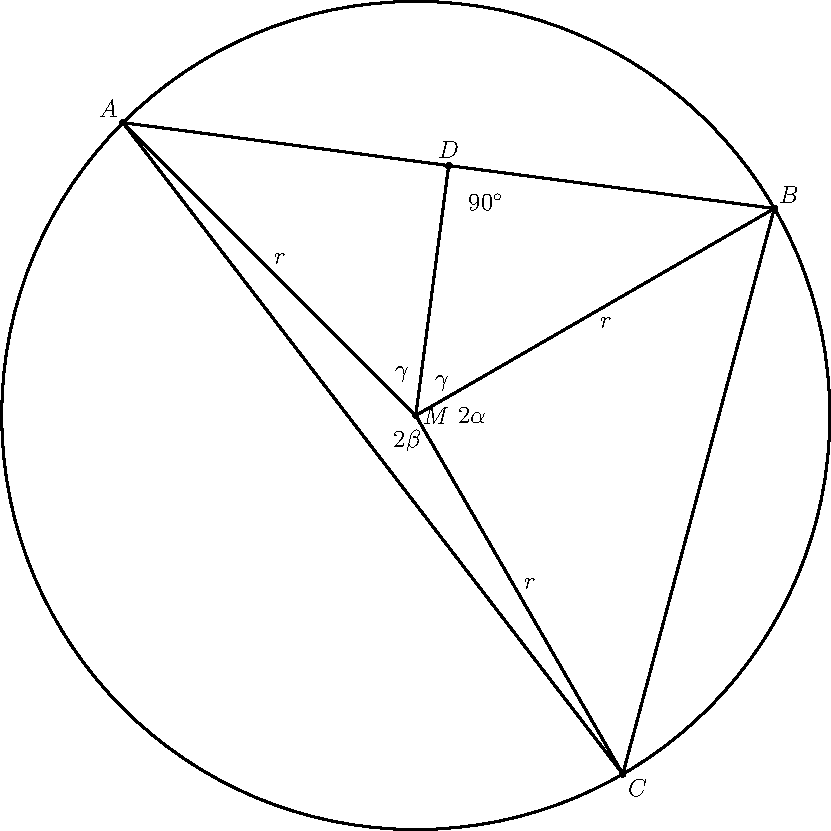
\includegraphics[scale=.5]{./sinelaw.pdf}
  \end{figure}
\end{frame}

\begin{frame}
  \frametitle{Law of Sines}
A circumcircle exists because there is a point $M$ which is
    the intersection of the two lines going through the
    midpoints of $A,B$ and $B,C$, respectively, and being
    perpendicular to $AB$ and $BC$, respectively.
    $\overline{MA}=\overline{MB}$ and $\overline{MB}=\overline{MC}$
    because of the way we have constructed $M$. Therefore
    $\overline{MA}=\overline{MC}$ so that the circle around $M$ going
    through $A$ and $B$ also goes through $C$.
\end{frame}

\begin{frame}
  \frametitle{Law of Sines}
  Consider the matrix
    \begin{equation}
      \label{eq:thiakohk}
    A=\left[
    \begin{array}{ccc}
      1&1&0 \\
       1&0&1 \\
       0&1&1
    \end{array}\right]
    \end{equation}
    It's inverse is
    \begin{equation}
      \label{eq:gajeerie}
      A^{-1}=\frac{1}{2}\left[
        \begin{array}{ccc}
          1&1&-1 \\
           1&-1&1 \\
           -1&1&1
        \end{array}\right]
    \end{equation}
\end{frame}

\begin{frame}
  \frametitle{Law of Sines}
    Use the fact that $ABM,BCM,ACM$ are isosceles triangles for
    \begin{equation}
      \label{eq:exiebohc}
      A\cdot\left[\begin{array}{c}
        \psi \\
              \phi \\
              \theta
            \end{array}\right]=\left[
            \begin{array}{c}
              360^{\circ}-2\alpha \\
              360^{\circ}-2\beta \\
              360^{\circ}-2\gamma \\
            \end{array}\right]
        \end{equation}
        where $\theta=\angle{}BMC,\phi=\angle{}AMC,\psi=\angle{}AMB$.
        Then
        \begin{equation}
          \label{eq:taineich}
          \left[\begin{array}{c}
        \psi \\
              \phi \\
              \theta
            \end{array}\right]=A^{-1}\cdot\left[
            \begin{array}{c}
              360^{\circ}-2\alpha \\
              360^{\circ}-2\beta \\
              360^{\circ}-2\gamma \\
            \end{array}\right]
        \end{equation}
        establishing that $\theta=2\alpha,\phi=2\beta,\psi=2\gamma$.
\end{frame}

\begin{frame}
  \frametitle{Law of Cosines}
Draw the height of a triangle (for example, at $B$) and call it $h$.
Let its foot on the side $b$ be called $D$. Let $x$ be the segment from
$A$ to $D$. Note that
\begin{equation}
  \label{eq:ohchuach}
  x^{2}+h^{2}=c^{2}
\end{equation}
and
\begin{equation}
  \label{eq:iepoohie}
  x=c\cdot\cos{}\alpha
\end{equation}
(\ref{eq:ohchuach}) and (\ref{eq:iepoohie}) substituted in
\begin{equation}
  \label{eq:uezaique}
  a^{2}=(b-x)^{2}+h^{2}
\end{equation}
give us the \alert{law of cosines}
\begin{equation}
  \label{eq:aiwugith}
  a^{2}=b^{2}-2bx+(x^{2}+h^{2})=b^{2}+c^{2}-2bc\cdot\cos\alpha
\end{equation}
\end{frame}

\begin{frame}
  \frametitle{Definition of Inverse Trigonometric Functions}
  Here is a formal definition of the arcsin function.
  \begin{block}{Arcsin Function}
    $\arcsin:[-1,1]\rightarrow\mathbb{R}$ such that
    \begin{equation}
      \label{eq:xaeshaut}
    \arcsin(x)=\vartheta\mbox{ if and only if }\sin\vartheta=x\mbox{
      and }-90^{\circ}\leq\vartheta\leq{}90^{\circ}\notag
    \end{equation}
  \end{block}

  \bigskip
  
  \begin{itemize}
  \item $\arcsin:[-1,1]\rightarrow\mathbb{R}$ has a range of $[-90^{\circ},90^{\circ}]$.
  \item $\arccos:[-1,1]\rightarrow\mathbb{R}$ is defined similarly
with a range of $[0^{\circ},180^{\circ}]$.
\item $\arctan:\mathbb{R}\rightarrow\mathbb{R}$ is defined similarly
with a range of $[-90^{\circ},90^{\circ}]$.
\item $\arctan:\mathbb{R}\rightarrow\mathbb{R}$ is defined similarly
with a range of $[0^{\circ},180^{\circ}]$.
  \end{itemize}
\end{frame}

% \begin{frame}
%   \frametitle{Applying the Laws of Sines/Cosines}
%   When you use the law of sines, you may have to use the arcsin
%   function. The range of the arcsin function is
%   $[-90^{\circ},90^{\circ}]$. For a triangle, however, the obtuse
%   solution for the equation $\sin\vartheta=x$ ($x$ is known) is also
%   relevant! Remember the following when you solve triangles using the
%   law of sines and the law of cosines.
% \end{frame}

\begin{frame}
  \frametitle{Applying the Laws of Sines/Cosines}
  \begin{description}
  \item[SSS] Use the law of cosines to find an angle. Make sure to
    solve for the largest angle (across from the longest side) first,
    or else a subsequent application of the law of sines may give you
    an incorrect result!
  \item[SAS] Use the law of cosines to find the missing side. Then (if
    you are using the law of sines) make sure to solve for the smaller
    angle (across from the shorter side) first, or else the law of
    sines may give you an incorrect result!
  \item[SSA] Use the law of sines. Consider both the acute \alert{and
      the obtuse} solution suggested by the arcsin function. 
  \item[AAS] (Any two angles and one side.) Calculate the third angle
    using the triangle postulate (the three angles add up to
    $180^{\circ}$). Then use the law of sines.
  \end{description}
\end{frame}

\begin{frame}
  \frametitle{Law of Sines Scenarios}
      \begin{figure}[h]
    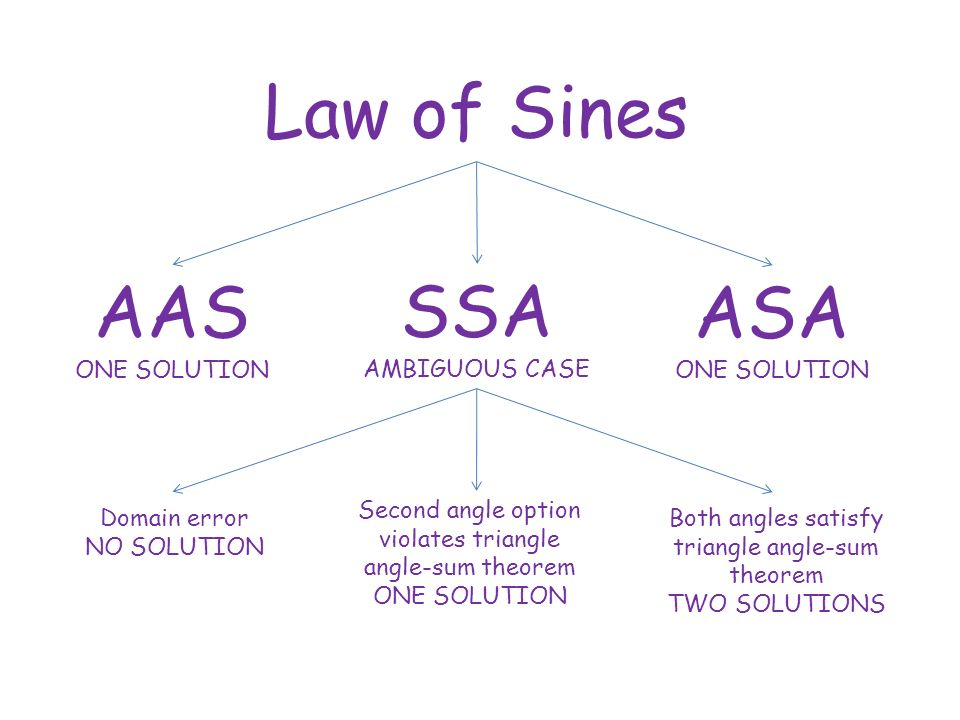
\includegraphics[scale=.4]{./law_of_sines_cases.jpg}
  \end{figure}
\end{frame}

\begin{frame}
  \frametitle{Law of Cosines Scenarios}
      \begin{figure}[h]
    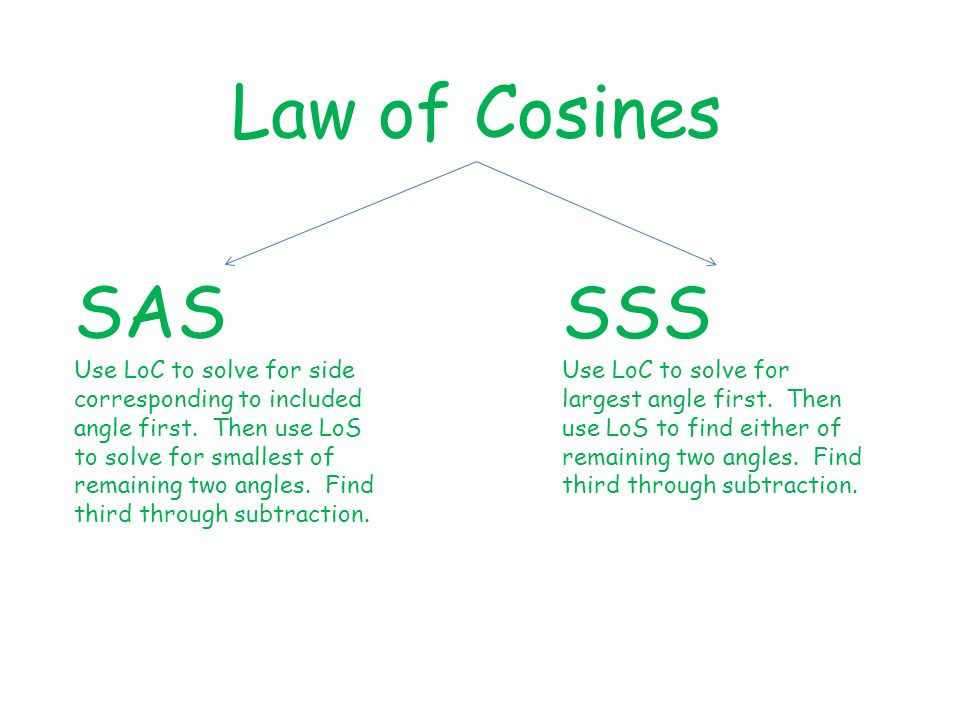
\includegraphics[scale=.4]{./law_of_cosines_cases.jpg}
  \end{figure}
\end{frame}

\begin{frame}
  \frametitle{Exercises}
{\ubung}  Solve the following triangle. $\alpha=23^{\circ},a=7in,c=10in$.
  ($\alpha$ is the acute angle on the bottom. Vertices are labeled
  clockwise.)
  \begin{figure}[h]
    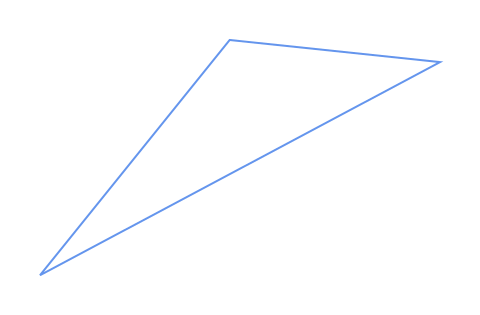
\includegraphics[scale=.5]{./LawOfSines3.png}
  \end{figure}
\end{frame}

\begin{frame}
  \frametitle{Exercises}
{\ubung} Solve the following triangle. $\gamma=28^{\circ},a=80.221m,c=46.112m$.
  \begin{figure}[h]
    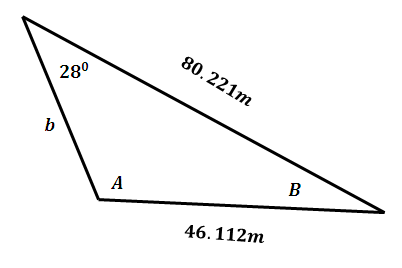
\includegraphics[scale=.5]{./LawOfSines1.png}
  \end{figure}
\end{frame}

\begin{frame}
  \frametitle{Exercises}
{\ubung} Solve the triangle in the diagram.
  \begin{figure}[h]
    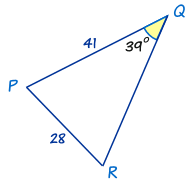
\includegraphics[scale=.75]{./LawOfSines4.png}
  \end{figure}
\end{frame}

\begin{frame}
  \frametitle{Exercises}
Note that there are two possible answers in this case. There are only
two possible answers in the scenario where you are given two sides and
an angle that is \alert{not} between the two sides.
  \begin{figure}[h]
    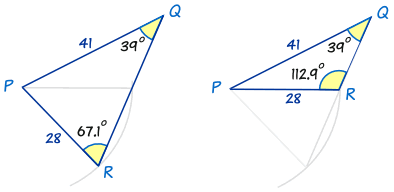
\includegraphics[scale=.5]{./LawOfSines5.png}
  \end{figure}
\end{frame}

\begin{frame}
  \frametitle{Exercises}
{\ubung} Solve the following triangle. $a=60.223m,b=37.876m,c=41.303m$.
  \begin{figure}[h]
    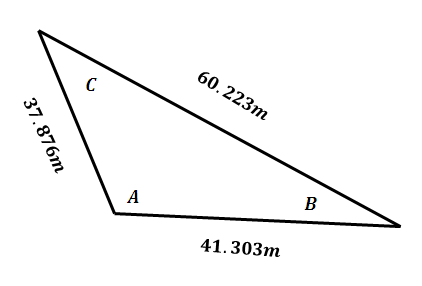
\includegraphics[scale=.5]{./LawOfSines2.png}
  \end{figure}
\end{frame}

\begin{frame}
  \frametitle{Law of Cosines Nota Bene}
  Solve for the \alert{largest angle first}! The cosine is one-to-one
  on the domain $[0^{\circ},180^{\circ}]$, so the arccosine will give
  you a unique result and correctly identify an obtuse angle. If you
  solve for a smaller angle first and then use the law of sines to
  find the obtuse angle, the arcsine will give you the acute angle
  instead of the obtuse one. Alternatively, you can always use the law
  of cosines and not get any ambiguities.
  % The arcsine of a number
  % between 0 and 1 usually has two solutions, so it is when we use the
  % law of sines that we need to be careful.
\end{frame}

\begin{frame}
  \frametitle{Exercises}
{\ubung} Solve the triangle in the diagram.
  \begin{figure}[h]
    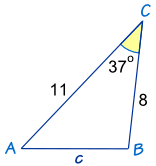
\includegraphics[scale=.75]{./LawOfSines6.png}
  \end{figure}
\end{frame}

\begin{frame}
  \frametitle{Exercises}
  {\ubung} Solve the following triangles.
  \begin{enumerate}
  \item $a=11,b=6,c=7$
  \item $b=0.49,c=0.98,\alpha=19^{\circ}$
  \item $b=8,c=7,\beta=48^{\circ}$
  \item $a=211,\beta=96^{\circ}14'51'',\gamma=31^{\circ}1'40''$
  \end{enumerate}
\end{frame}

\begin{frame}
  \frametitle{End of Lesson}
Next Lesson: Quadratic Equations
\end{frame}

\end{document}
